% Options for packages loaded elsewhere
\PassOptionsToPackage{unicode}{hyperref}
\PassOptionsToPackage{hyphens}{url}
%
\documentclass[
]{article}
\usepackage{amsmath,amssymb}
\usepackage{lmodern}
\usepackage{iftex}
\ifPDFTeX
  \usepackage[T1]{fontenc}
  \usepackage[utf8]{inputenc}
  \usepackage{textcomp} % provide euro and other symbols
\else % if luatex or xetex
  \usepackage{unicode-math}
  \defaultfontfeatures{Scale=MatchLowercase}
  \defaultfontfeatures[\rmfamily]{Ligatures=TeX,Scale=1}
\fi
% Use upquote if available, for straight quotes in verbatim environments
\IfFileExists{upquote.sty}{\usepackage{upquote}}{}
\IfFileExists{microtype.sty}{% use microtype if available
  \usepackage[]{microtype}
  \UseMicrotypeSet[protrusion]{basicmath} % disable protrusion for tt fonts
}{}
\makeatletter
\@ifundefined{KOMAClassName}{% if non-KOMA class
  \IfFileExists{parskip.sty}{%
    \usepackage{parskip}
  }{% else
    \setlength{\parindent}{0pt}
    \setlength{\parskip}{6pt plus 2pt minus 1pt}}
}{% if KOMA class
  \KOMAoptions{parskip=half}}
\makeatother
\usepackage{xcolor}
\IfFileExists{xurl.sty}{\usepackage{xurl}}{} % add URL line breaks if available
\IfFileExists{bookmark.sty}{\usepackage{bookmark}}{\usepackage{hyperref}}
\hypersetup{
  hidelinks,
  pdfcreator={LaTeX via pandoc}}
\urlstyle{same} % disable monospaced font for URLs
\usepackage[margin=1in]{geometry}
\usepackage{color}
\usepackage{fancyvrb}
\newcommand{\VerbBar}{|}
\newcommand{\VERB}{\Verb[commandchars=\\\{\}]}
\DefineVerbatimEnvironment{Highlighting}{Verbatim}{commandchars=\\\{\}}
% Add ',fontsize=\small' for more characters per line
\usepackage{framed}
\definecolor{shadecolor}{RGB}{248,248,248}
\newenvironment{Shaded}{\begin{snugshade}}{\end{snugshade}}
\newcommand{\AlertTok}[1]{\textcolor[rgb]{0.94,0.16,0.16}{#1}}
\newcommand{\AnnotationTok}[1]{\textcolor[rgb]{0.56,0.35,0.01}{\textbf{\textit{#1}}}}
\newcommand{\AttributeTok}[1]{\textcolor[rgb]{0.77,0.63,0.00}{#1}}
\newcommand{\BaseNTok}[1]{\textcolor[rgb]{0.00,0.00,0.81}{#1}}
\newcommand{\BuiltInTok}[1]{#1}
\newcommand{\CharTok}[1]{\textcolor[rgb]{0.31,0.60,0.02}{#1}}
\newcommand{\CommentTok}[1]{\textcolor[rgb]{0.56,0.35,0.01}{\textit{#1}}}
\newcommand{\CommentVarTok}[1]{\textcolor[rgb]{0.56,0.35,0.01}{\textbf{\textit{#1}}}}
\newcommand{\ConstantTok}[1]{\textcolor[rgb]{0.00,0.00,0.00}{#1}}
\newcommand{\ControlFlowTok}[1]{\textcolor[rgb]{0.13,0.29,0.53}{\textbf{#1}}}
\newcommand{\DataTypeTok}[1]{\textcolor[rgb]{0.13,0.29,0.53}{#1}}
\newcommand{\DecValTok}[1]{\textcolor[rgb]{0.00,0.00,0.81}{#1}}
\newcommand{\DocumentationTok}[1]{\textcolor[rgb]{0.56,0.35,0.01}{\textbf{\textit{#1}}}}
\newcommand{\ErrorTok}[1]{\textcolor[rgb]{0.64,0.00,0.00}{\textbf{#1}}}
\newcommand{\ExtensionTok}[1]{#1}
\newcommand{\FloatTok}[1]{\textcolor[rgb]{0.00,0.00,0.81}{#1}}
\newcommand{\FunctionTok}[1]{\textcolor[rgb]{0.00,0.00,0.00}{#1}}
\newcommand{\ImportTok}[1]{#1}
\newcommand{\InformationTok}[1]{\textcolor[rgb]{0.56,0.35,0.01}{\textbf{\textit{#1}}}}
\newcommand{\KeywordTok}[1]{\textcolor[rgb]{0.13,0.29,0.53}{\textbf{#1}}}
\newcommand{\NormalTok}[1]{#1}
\newcommand{\OperatorTok}[1]{\textcolor[rgb]{0.81,0.36,0.00}{\textbf{#1}}}
\newcommand{\OtherTok}[1]{\textcolor[rgb]{0.56,0.35,0.01}{#1}}
\newcommand{\PreprocessorTok}[1]{\textcolor[rgb]{0.56,0.35,0.01}{\textit{#1}}}
\newcommand{\RegionMarkerTok}[1]{#1}
\newcommand{\SpecialCharTok}[1]{\textcolor[rgb]{0.00,0.00,0.00}{#1}}
\newcommand{\SpecialStringTok}[1]{\textcolor[rgb]{0.31,0.60,0.02}{#1}}
\newcommand{\StringTok}[1]{\textcolor[rgb]{0.31,0.60,0.02}{#1}}
\newcommand{\VariableTok}[1]{\textcolor[rgb]{0.00,0.00,0.00}{#1}}
\newcommand{\VerbatimStringTok}[1]{\textcolor[rgb]{0.31,0.60,0.02}{#1}}
\newcommand{\WarningTok}[1]{\textcolor[rgb]{0.56,0.35,0.01}{\textbf{\textit{#1}}}}
\usepackage{graphicx}
\makeatletter
\def\maxwidth{\ifdim\Gin@nat@width>\linewidth\linewidth\else\Gin@nat@width\fi}
\def\maxheight{\ifdim\Gin@nat@height>\textheight\textheight\else\Gin@nat@height\fi}
\makeatother
% Scale images if necessary, so that they will not overflow the page
% margins by default, and it is still possible to overwrite the defaults
% using explicit options in \includegraphics[width, height, ...]{}
\setkeys{Gin}{width=\maxwidth,height=\maxheight,keepaspectratio}
% Set default figure placement to htbp
\makeatletter
\def\fps@figure{htbp}
\makeatother
\setlength{\emergencystretch}{3em} % prevent overfull lines
\providecommand{\tightlist}{%
  \setlength{\itemsep}{0pt}\setlength{\parskip}{0pt}}
\setcounter{secnumdepth}{-\maxdimen} % remove section numbering
\usepackage{graphicx}				% Use pdf, png, jpg, or eps§ with pdflatex; use eps in DVI mode
\usepackage{amsmath}
\usepackage{natbib}
\usepackage{bm}
\usepackage{ctable}
\usepackage{setspace}
\usepackage{enumitem}
\usepackage{geometry}
% \usepackage{fancyhdr}
% \pagestyle{fancy}
% % header
% % \fancyhead[LO,LE]{Liz Lawler}
% \fancyhead[CO,CE]{Naveau Distributions}
% \fancyhead[RO,RE]{December 17, 2021}
\newlist{longenum}{enumerate}{3}
\setlist[longenum,1]{label=\arabic*.}
\setlist[longenum,2]{label=(\alph*)}
\setlist[longenum,3]{label=\roman*)}
% \usepackage{xcolor}
% \usepackage{newtxtext} % Times-like font
% \usepackage{titlesec}
% \titleformat*{\section}{\Large\bfseries\sffamily}
% \titleformat*{\subsection}{\large\bfseries\sffamily}



%%%%%%%%%%%
% Math Macros
\newcommand{\bmA}{\ensuremath{\bm A}}
\newcommand{\bma}{\ensuremath{\bm a}}
\newcommand{\bmB}{\ensuremath{\bm B}}
\newcommand{\bmb}{\ensuremath{\bm b}}
\newcommand{\bmC}{\ensuremath{\bm C}}
\newcommand{\bmc}{\ensuremath{\bm c}}
\newcommand{\bmD}{\ensuremath{\bm D}}
\newcommand{\bmd}{\ensuremath{\bm d}}
\newcommand{\bme}{\ensuremath{\bm e}}
\newcommand{\bmE}{\ensuremath{\bm E}}
\newcommand{\bmF}{\ensuremath{\bm F}}
\newcommand{\bmG}{\ensuremath{\bm G}}
\newcommand{\bmg}{\ensuremath{\bm g}}
\newcommand{\bmH}{\ensuremath{\bm H}}
\newcommand{\bmI}{\ensuremath{\bm I}}
\newcommand{\bmJ}{\ensuremath{\bm J}}
\newcommand{\bmL}{\ensuremath{\bm L}}
\newcommand{\bmM}{\ensuremath{\bm M}}
\newcommand{\bmP}{\ensuremath{\bm P}}
\newcommand{\bmQ}{\ensuremath{\bm Q}}
\newcommand{\bmq}{\ensuremath{\bm q}}
\newcommand{\bmR}{\ensuremath{\bm R}}
\newcommand{\bmr}{\ensuremath{\bm r}}
\newcommand{\bmS}{\ensuremath{\bm S}}
\newcommand{\bmt}{\ensuremath{\bm t}}
\newcommand{\bmU}{\ensuremath{\bm U}}
\newcommand{\bmu}{\ensuremath{\bm u}}
\newcommand{\bmV}{\ensuremath{\bm V}}
\newcommand{\bmv}{\ensuremath{\bm v}}
\newcommand{\bmW}{\ensuremath{\bm W}}
\newcommand{\bmw}{\ensuremath{\bm w}}
\newcommand{\bmX}{\ensuremath{\bm X}}
\newcommand{\bmx}{\ensuremath{\bm x}}
\newcommand{\bmY}{\ensuremath{\bm Y}}
\newcommand{\bmy}{\ensuremath{\bm y}}
\newcommand{\bmZ}{\ensuremath{\bm Z}}
\newcommand{\bmz}{\ensuremath{\bm z}}



\newcommand{\bmalpha}{\ensuremath{\bm{\alpha}}}
\newcommand{\bmbeta}{\ensuremath{\bm{\beta}}}
\newcommand{\bmdelta}{\ensuremath{\bm{\delta}}}
\newcommand{\bmepsilon}{\ensuremath{\bm{\epsilon}}}
\newcommand{\bmGamma}{\ensuremath{\bm{\Gamma}}}
\newcommand{\bmLambda}{\ensuremath{\bm{\Lambda}}}
\newcommand{\bmmu}{\ensuremath{\bm{\mu}}}
\newcommand{\bmSigma}{\ensuremath{\bm{\Sigma}}}
\newcommand{\bmzeta}{\ensuremath{\bm{\zeta}}}


\newcommand{\rank}{\ensuremath{\mathsf{rank}}}
\newcommand{\nullity}{\ensuremath{\mathsf{nullity}}}
\newcommand{\trace}{\ensuremath{\mathsf{tr}}}
\newcommand{\diag}{\ensuremath{\mathsf{diag}}}
\newcommand{\vecspan}{\ensuremath{\mathsf{span}}}

\newcommand{\mT}{\ensuremath{\mathsf{T}}}
\newcommand{\indep}{\perp \!\!\! \perp}

\newcommand{\bbh}{\ensuremath{\hat{\bmbeta}}}
\newcommand{\bhy}{\ensuremath{\hat{\bmY}}}
\newcommand{\Rn}{\ensuremath{\mathbb{R}^n}}
\newcommand{\Rnp}{\ensuremath{\mathbb{R}^{n\times p}}}
\newcommand{\Pv}{\ensuremath{{\bmP}_\mathcal{V}}}
\newcommand{\Pw}{\ensuremath{{\bmP}_\mathcal{W}}}
\newcommand{\Px}{\ensuremath{{\bmP}_{\bmX}}}
\newcommand{\Pd}{\ensuremath{{\bmP}_{\bmd}}}
\newcommand{\XtX}{\ensuremath{\bmX^\mT\bmX}}
\newcommand{\XtXinv}{\ensuremath{(\bmX^\mT\bmX)^{-1}}}
\newcommand{\XtXg}{\ensuremath{(\bmX^\mT\bmX)^{-}}}
\newcommand{\gtb}{\ensuremath{\bmg^\mT\bmbeta}}
\newcommand{\Jn}{\ensuremath{{\bmJ}_n}}
\newcommand{\Vcal}{\ensuremath{\mathcal{V}}}
\newcommand{\Vperp}{\ensuremath{\mathcal{V}^\perp}}
\newcommand{\Wcal}{\ensuremath{\mathcal{W}}}

\DeclareMathOperator*{\argmin}{arg\,min}
\newcommand{\bbmx}{\ensuremath{\begin{bmatrix}}}
\newcommand{\ebmx}{\ensuremath{\end{bmatrix}}}
\newcommand{\ealn}{\ensuremath{\end{aligned}}}
\newcommand{\baln}{\ensuremath{\begin{aligned}}}

\newcommand{\E}{\ensuremath{\mathrm{E}}}
\newcommand{\Var}{\ensuremath{\mathrm{Var}}}
\newcommand{\SE}{\ensuremath{\mathrm{SE}}}
\newcommand{\Cov}{\ensuremath{\mathrm{Cov}}}
\newcommand{\Bias}{\ensuremath{\mathrm{Bias}}}


\newcommand{\FWER}{\ensuremath{\mathrm{FWER}}}
\newcommand{\PCER}{\ensuremath{\mathrm{PCER}}}
\newcommand{\FDR}{\ensuremath{\mathrm{FDR}}}
\newcommand{\sFWER}{\ensuremath{\mathrm{sFWER}}}
\newcommand{\diet}{\ensuremath{\mathrm{diet}}}

\newcommand{\F}{\ensuremath{\mathrm{F}}}

\newcommand{\benum}{\begin{enumerate}}
\newcommand{\eenum}{\begin{enumerate}}

\newcommand{\blonge}{\begin{longenum}}
\newcommand{\elonge}{\end{longenum}}
\ifLuaTeX
  \usepackage{selnolig}  % disable illegal ligatures
\fi

\author{}
\date{\vspace{-2.5em}}

\begin{document}

\hypertarget{general-form-of-distributions}{%
\subsubsection{General Form of
Distributions}\label{general-form-of-distributions}}

\[F(x) = G\{H_{\xi}{(\frac{x}{\sigma})} \} \]

\hypertarget{parametric-families}{%
\subsubsection{Parametric Families}\label{parametric-families}}

\begin{enumerate}
\def\labelenumi{\arabic{enumi}.}
\tightlist
\item
  \(G(v) = v^\kappa, \ \kappa > 0\)
  \[F_1(x) = \{1 - [1 + \xi(\frac{x}{\sigma})]^{-1/\xi} \}^\kappa\]
  \[f_1(x) = \frac{\kappa}{\sigma}[1 + \xi (\frac{x}{\sigma})]^{-(1/\xi + 1)}\{1 - [1+\xi(\frac{x}{\sigma})]^{-1/\xi} \} ^{\kappa-1}\]
\end{enumerate}

\begin{center}\includegraphics[width=0.6\linewidth]{dist_sheet_files/figure-latex/unnamed-chunk-1-1} \end{center}

\[F_1^{-1}(U) = \frac{\sigma}{\xi} [(1-U^{1/\kappa})^{-\xi} - 1]\]

\begin{enumerate}
\def\labelenumi{\arabic{enumi}.}
\setcounter{enumi}{1}
\tightlist
\item
  \(G(v) = pv^{\kappa_1} + (1-p)v^{\kappa_2}, \ \kappa_1, \kappa_2 >0\)
  \[F_2(x) = p\{1 - [1 + \xi(\frac{x}{\sigma})]^{-1/\xi} \}^{\kappa_1} + (1-p)\{1 - [1 + \xi(\frac{x}{\sigma})]^{-1/\xi} \}^{\kappa_2}\]
  \[f_2(x) = \frac{1}{\sigma}[1 + \xi (\frac{x}{\sigma})]^{-(1/\xi + 1)}\left(\kappa_1p\{1 - [1+\xi(\frac{x}{\sigma})]^{-1/\xi} \} ^{\kappa_1-1} + \kappa_2(1-p)\{1 - [1+\xi(\frac{x}{\sigma})]^{-1/\xi} \} ^{\kappa_2-1}\right)\]
\end{enumerate}

\begin{center}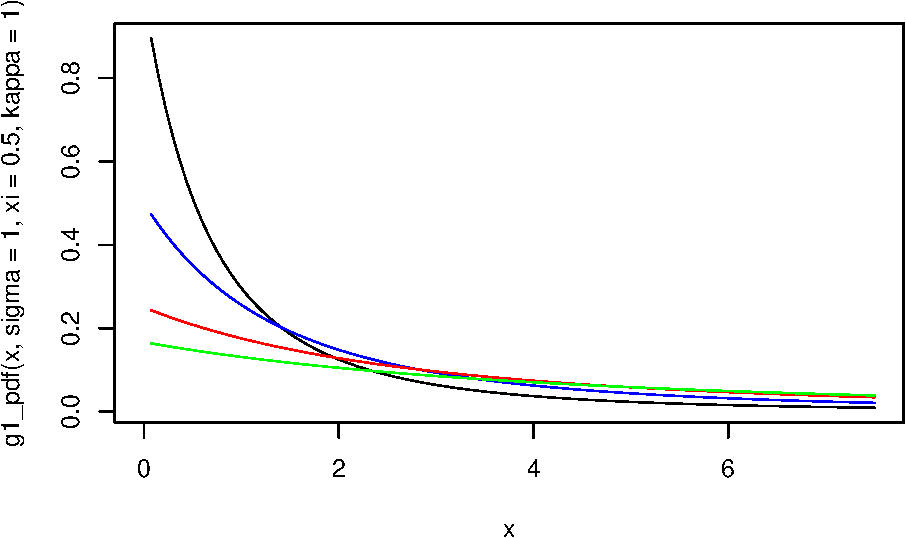
\includegraphics[width=0.6\linewidth]{dist_sheet_files/figure-latex/unnamed-chunk-4-1} \end{center}

\pagebreak

\begin{enumerate}
\def\labelenumi{\arabic{enumi}.}
\setcounter{enumi}{2}
\tightlist
\item
  \(G(v) = 1-Q_\delta\{(1-v)^\delta\}, \ \delta > 0, \ \ Q_\delta \sim \text{Beta}(1/\delta, 2)\)
  \[F_3(x) = 1 - Q_\delta\{[1 + \xi(\frac{x}{\sigma})]^{-\delta/\xi} \}, \ \ Q_\delta \stackrel{d}{=}\text{Beta}(1/\delta, 2)\]
\end{enumerate}

\[f_3(x) = \frac{1 + \delta}{\delta\sigma}[1 + \xi (\frac{x}{\sigma})]^{-(1/\xi + 1)}\left(1 - [1+\xi(\frac{x}{\sigma})]^{-\delta/\xi} \right)\]

\begin{Shaded}
\begin{Highlighting}[]
\NormalTok{g3\_pdf }\OtherTok{\textless{}{-}} \ControlFlowTok{function}\NormalTok{(x, }\AttributeTok{sigma =}\NormalTok{ sigma, }\AttributeTok{xi =}\NormalTok{ xi, }\AttributeTok{delta =}\NormalTok{ delta) \{}
\NormalTok{    lpdf }\OtherTok{\textless{}{-}} \FunctionTok{log}\NormalTok{(}\DecValTok{1} \SpecialCharTok{+}\NormalTok{ delta) }\SpecialCharTok{{-}} \FunctionTok{log}\NormalTok{(delta }\SpecialCharTok{*}\NormalTok{ sigma) }\SpecialCharTok{{-}}\NormalTok{ (}\DecValTok{1}\SpecialCharTok{/}\NormalTok{xi }\SpecialCharTok{+} \DecValTok{1}\NormalTok{) }\SpecialCharTok{*}
        \FunctionTok{log}\NormalTok{(}\DecValTok{1} \SpecialCharTok{+}\NormalTok{ xi }\SpecialCharTok{*}\NormalTok{ (x}\SpecialCharTok{/}\NormalTok{sigma)) }\SpecialCharTok{+} \FunctionTok{log}\NormalTok{(}\DecValTok{1} \SpecialCharTok{{-}}\NormalTok{ (}\DecValTok{1} \SpecialCharTok{+}\NormalTok{ xi }\SpecialCharTok{*}\NormalTok{ (x}\SpecialCharTok{/}\NormalTok{sigma))}\SpecialCharTok{\^{}}\NormalTok{(}\SpecialCharTok{{-}}\NormalTok{delta}\SpecialCharTok{/}\NormalTok{xi))}
    \FunctionTok{return}\NormalTok{(}\FunctionTok{exp}\NormalTok{(lpdf))}
\NormalTok{\}}
\end{Highlighting}
\end{Shaded}

\begin{Shaded}
\begin{Highlighting}[]
\FunctionTok{curve}\NormalTok{(}\FunctionTok{g3\_pdf}\NormalTok{(x, }\AttributeTok{sigma =} \DecValTok{1}\NormalTok{, }\AttributeTok{xi =} \FloatTok{0.5}\NormalTok{, }\AttributeTok{delta =} \DecValTok{25}\NormalTok{), }\AttributeTok{xlim =} \FunctionTok{c}\NormalTok{(}\DecValTok{0}\NormalTok{,}
    \DecValTok{7}\NormalTok{), }\AttributeTok{ylim =} \FunctionTok{c}\NormalTok{(}\DecValTok{0}\NormalTok{, }\DecValTok{1}\NormalTok{), }\AttributeTok{ylab =} \StringTok{"pdf"}\NormalTok{, }\AttributeTok{col =} \StringTok{"red"}\NormalTok{)}
\FunctionTok{curve}\NormalTok{(}\FunctionTok{g3\_pdf}\NormalTok{(x, }\AttributeTok{sigma =} \DecValTok{1}\NormalTok{, }\AttributeTok{xi =} \FloatTok{0.5}\NormalTok{, }\AttributeTok{delta =} \DecValTok{5}\NormalTok{), }\AttributeTok{xlim =} \FunctionTok{c}\NormalTok{(}\DecValTok{0}\NormalTok{,}
    \DecValTok{7}\NormalTok{), }\AttributeTok{add =} \ConstantTok{TRUE}\NormalTok{, }\AttributeTok{col =} \StringTok{"blue"}\NormalTok{)}
\FunctionTok{curve}\NormalTok{(}\FunctionTok{g3\_pdf}\NormalTok{(x, }\AttributeTok{sigma =} \DecValTok{1}\NormalTok{, }\AttributeTok{xi =} \FloatTok{0.5}\NormalTok{, }\AttributeTok{delta =} \DecValTok{3}\NormalTok{), }\AttributeTok{xlim =} \FunctionTok{c}\NormalTok{(}\DecValTok{0}\NormalTok{,}
    \DecValTok{7}\NormalTok{), }\AttributeTok{add =} \ConstantTok{TRUE}\NormalTok{, }\AttributeTok{col =} \StringTok{"green"}\NormalTok{)}
\end{Highlighting}
\end{Shaded}

\begin{center}\includegraphics[width=0.6\linewidth]{dist_sheet_files/figure-latex/unnamed-chunk-15-1} \end{center}

\[F_3^{-1}(U) = \frac{\sigma}{\xi}\left([Q_\delta^{-1}\{1 - U\}]^{-\xi/\delta} - 1\right)\]

\begin{Shaded}
\begin{Highlighting}[]
\NormalTok{g3\_cdf\_inv }\OtherTok{\textless{}{-}} \ControlFlowTok{function}\NormalTok{(u, }\AttributeTok{sigma =}\NormalTok{ sigma, }\AttributeTok{xi =}\NormalTok{ xi, }\AttributeTok{delta =}\NormalTok{ delta) \{}
\NormalTok{    (sigma}\SpecialCharTok{/}\NormalTok{xi) }\SpecialCharTok{*}\NormalTok{ ((}\FunctionTok{qbeta}\NormalTok{((}\DecValTok{1} \SpecialCharTok{{-}}\NormalTok{ u), (}\DecValTok{1}\SpecialCharTok{/}\NormalTok{delta), }\DecValTok{2}\NormalTok{)}\SpecialCharTok{\^{}}\NormalTok{(}\SpecialCharTok{{-}}\NormalTok{xi}\SpecialCharTok{/}\NormalTok{delta)) }\SpecialCharTok{{-}}
        \DecValTok{1}\NormalTok{)}
\NormalTok{\}}

\NormalTok{g3\_rng }\OtherTok{\textless{}{-}} \ControlFlowTok{function}\NormalTok{(n, }\AttributeTok{sigma =}\NormalTok{ sigma, }\AttributeTok{xi =}\NormalTok{ xi, }\AttributeTok{delta =}\NormalTok{ delta) \{}
    \FunctionTok{g3\_cdf\_inv}\NormalTok{(}\FunctionTok{runif}\NormalTok{(n), sigma, xi, delta)}
\NormalTok{\}}
\end{Highlighting}
\end{Shaded}

\pagebreak

\(\delta = 1\)

\begin{center}\includegraphics[width=0.6\linewidth]{dist_sheet_files/figure-latex/unnamed-chunk-17-1} \end{center}

\(\delta = 3\)

\begin{center}\includegraphics[width=0.6\linewidth]{dist_sheet_files/figure-latex/unnamed-chunk-18-1} \end{center}

\(\delta = 5\)

\begin{center}\includegraphics[width=0.6\linewidth]{dist_sheet_files/figure-latex/unnamed-chunk-19-1} \end{center}

\begin{enumerate}
\def\labelenumi{\arabic{enumi}.}
\setcounter{enumi}{3}
\tightlist
\item
  \(G(v) = [1-Q_\delta\{(1-v)^\delta\}]^{\kappa/2}, \ \kappa, \delta > 0\)
  \[F_4(x) = [1 - Q_\delta\{[1 + \xi(\frac{x}{\sigma})]^{-\delta/\xi} \}]^{\kappa/2}, \ \ Q_\delta \stackrel{d}{=}\text{Beta}(1/\delta, 2)\]
\end{enumerate}

\end{document}
